\documentclass[11pt]{article}


\usepackage[sort]{natbib}
\usepackage{bm,amsmath,bbm,amsfonts,nicefrac,latexsym,amsmath,amsfonts,amsbsy,amscd,amsxtra,amsgen,amsopn,bbm,amsthm,amssymb,graphicx}
\usepackage{fancyhdr}
\usepackage{caption}
\usepackage{subcaption}
\usepackage[margin=1.0in]{geometry}


\title{Information content for observations of forest carbon stocks and fluxes when assimilated with the DALEC carbon balance model}
%\date{\normalsize{3$^{\text{rd}}$ June 2014, \ Room 1L36}}
\author{\normalsize{E. Pinnington}}


\newtheorem{theorem}{Theorem}[section]
\newtheorem*{defn}{Definition}

	
\begin{document}

\maketitle

\section*{Shannon Information Content}

In DA Shannon Information Content ($SIC$) is a measure of the reduction in entropy given a set of observations. Entropy physically corresponds to the volume in state space taken up by the probability density function (pdf) describing the knowledge of the state \cite{rodgers2000inverse}. Assuming all pdfs are Gaussian we have,
\[
SIC=\frac{1}{2}ln\frac{\begin{vmatrix} \bf{B} \end{vmatrix}}{\begin{vmatrix} \bf{A} \end{vmatrix}},
\]
where $\bf{B}$ is the background error covariance matrix and $\bf{A}$ is the analysis error covariance matrix. For a larger reduction in uncertainty in our analysis we have a larger value of $SIC$. I began by using $SIC$ to understand the information content for different sets of observations at one time when being assimilated with the DALEC model. We specify the state vector for the assimilation as,
\[ \underline{x}_b = (C_f, C_r, C_w, C_l, C_s)^T, \] 
where the elements of the state vector have variances, $\sigma_{cf,b}^{2},\ldots,\sigma_{cs,b}^{2}$, respectively. We then have the following background error covariance matrix,
\[
\bf{B} = \begin{pmatrix} 
\sigma_{cf,b}^{2} & 0 & 0 & 0 & 0 \\
0 & \sigma_{cr,b}^{2} & 0 & 0 & 0 \\
0 & 0 & \sigma_{cw,b}^{2} & 0 & 0 \\
0 & 0 & 0 & \sigma_{cl,b}^{2} & 0 \\
0 & 0 & 0 & 0 & \sigma_{cs,b}^{2} \\
\end{pmatrix},
\]  
here we assume a diagonal background error covariance matrix. In order to calculate the $SIC$ we need $\begin{vmatrix} \textbf{A}^{-1} \end{vmatrix}$ we have,
\[
\textbf{A}^{-1}=\textbf{J}'' = \textbf{B}^{-1}+\textbf{H}^{T}\textbf{R}^{-1}\bf{H}, 
\]
where $\textbf{J}''$ is the Hessian of $\bf{J}$, the cost function to be minimized in Three-Dimensional Variational Data Assimilation (3D-Var), and $\bf{H}$ is the linearized observation operator. 

\subsection*{$SIC$ for a single observation at one time}

If we first consider one observation of $C_f$ (the first element of our state vector $\underline{x}$) an analytical expression for the $SIC$ can be derived using,
\[
\textbf{H}_{0} = \begin{pmatrix}
1 & 0 & 0 & 0 & 0
\end{pmatrix},
\] 
where $\textbf{H}_{0}=\frac{\delta C_f(t_0)}{\delta\underline{x}}$ is the linearized observation operator at time $t_0$. As we have a single observation at one time our observation error covariance matrix, $\bf{R}$, is just the variance of our observation of $C_f$, $\sigma_{cf,o}^{2}$, at time $t_0$. Therefore,
\[
\textbf{R}=\sigma_{cf,o}^{2}
\]  
and
\[
\begin{array} {lcl}
\textbf{J}'' &=& \textbf{B}^{-1}+\textbf{H}^{T}\textbf{R}^{-1}\bf{H} \\
&=& \begin{pmatrix} 
\sigma_{cf,b}^{-2}+\sigma_{cf,o}^{-2} & 0 & 0 & 0 & 0 \\
0 & \sigma_{cr,b}^{-2} & 0 & 0 & 0 \\
0 & 0 & \sigma_{cw,b}^{-2} & 0 & 0 \\
0 & 0 & 0 & \sigma_{cl,b}^{-2} & 0 \\
0 & 0 & 0 & 0 & \sigma_{cs,b}^{-2} \\
\end{pmatrix}.
\end{array}
\] 
We then have,
\[
SIC=\frac{1}{2}ln\frac{\begin{vmatrix} \textbf{B} \end{vmatrix}}{\begin{vmatrix} \textbf{A} \end{vmatrix}} = \frac{1}{2}ln\begin{vmatrix} \textbf{B} \end{vmatrix}\begin{vmatrix} \textbf{J}'' \end{vmatrix}.
\]
Hence,
\[
SIC = \frac{1}{2}ln\frac{(\sigma_{cf,o}^{2}+\sigma_{cf,b}^{2})}{\sigma_{cf,o}^{2}}
=\frac{1}{2}ln \bigg(1+\frac{\sigma_{cf,b}^{2}}{\sigma_{cf,o}^{2}}\bigg).
\]
***Here we see the SIC is dependant on the ratio between the two variances and this will be the same for all other carbon pool observations. Something about better depending on pool observed.*** 

One of the main observations made of the carbon balance of a forest at flux tower sites is the net ecosystem exchange ($NEE$) of CO$_{2}$, which can be estimated by DALEC as the difference between $GPP$ and the respiration of $C_l$ and $C_s$, giving,
\[ 
NEE(t)=-(1-p_2)GPP(C_f(t),\phi)+p_8C_lT(t)+p_9C_sT(t). 
\]
For a single observation of $NEE$ at one time, $t_0$, an analytical expression for the $SIC$ can be derived using,
\[
\textbf{H}_{0} = \begin{pmatrix}
-(1-p_{2})\zeta_0 & 0 & 0 & p_{8}T_{0} & p_{9}T_{0}
\end{pmatrix},
\]  
where $\zeta_0 = GPP'(C_f(t_0), \phi)$, $T_{0}=T(t_0)$ and $\textbf{H}_{0}=\frac{\delta NEE(t_0)}{\delta\underline{x}}$ is the linearized observation operator at time $t_0$. Again our observation error covariance matrix, $\bf{R}$, is just the variance of our observation of $NEE$, $\sigma_{nee,0}^{2}$, at time $t_0$. Therefore,
\[
\textbf{R}=\sigma_{nee,0}^{2}
\]  
and
\[
\begin{array} {lcl}
\textbf{J}'' &=& \textbf{B}^{-1}+\textbf{H}^{T}\textbf{R}^{-1}\bf{H} \\
&=& \begin{pmatrix} 
\sigma_{cf,b}^{-2}+\sigma_{nee,0}^{-2}(1-p_{2})^{2}\zeta_0^{2} & 0 & 0 & \sigma_{nee,0}^{-2}(1-p_{2})\zeta_0 p_{8}T_0 & \sigma_{nee,0}^{-2}(1-p_{2})\zeta_0 p_{9}T_0 \\
0 & \sigma_{cr,b}^{-2} & 0 & 0 & 0 \\
0 & 0 & \sigma_{cw,b}^{-2} & 0 & 0 \\
\sigma_{nee,0}^{-2}(1-p_{2})\zeta_0 p_{8}T_0 & 0 & 0 & \sigma_{cl,b}^{-2}+\sigma_{nee,0}^{-2}p_{8}^2 T_0^2 & \sigma_{nee,0}^{-2}p_{8}p_{9} T_0^2 \\
\sigma_{nee,0}^{-2}(1-p_{2})\zeta_0 p_{9}T_0 & 0 & 0 & \sigma_{nee,0}^{-2}p_{8}p_{9} T_0^2 & \sigma_{cs,b}^{-2}+\sigma_{nee,0}^{-2}p_{9}^2 T_0^2 \\
\end{pmatrix}.
\end{array}
\] 
We then have,
\[
SIC=\frac{1}{2}ln\frac{\begin{vmatrix} \textbf{B} \end{vmatrix}}{\begin{vmatrix} \textbf{A} \end{vmatrix}} = \frac{1}{2}ln\begin{vmatrix} \textbf{B} \end{vmatrix}\begin{vmatrix} \textbf{J}'' \end{vmatrix}.
\]
Hence,
\[
SIC = \frac{1}{2}ln\frac{(p_{2}-1)^{2}\zeta_0^{2}\sigma_{cf,b}^{2}+\sigma_{nee,0}^{2}+T_{0}^2(p_{9}^2\sigma_{cs,b}^2+p_8^2\sigma_{cl,b}^2)}{\sigma_{nee,0}^{2}}.
\]
If we assume that the variances and parameters here are fixed we can see that the size of the $SIC$ is dependent on the temperature term, $T_0$, and the square of the first derivative of $GPP$, $\zeta_0^{2}$. Generally, the value of $GPP$ (and its first derivative) is highest in summer with higher total daily irradiance and higher temperatures. We therefore have that there will be more information content in observations that are taken when temperatures are higher. ***Physically this makes sense as more NEE takes place when temperatures are higher (to a point) so measurements are of greater magnitude and give us more information of carbon fluxes***. By plotting the SIC for a single observation of NEE varying with three years of meteorological driving data and the temperature term for the same period of the same data we can see that both are closely linked \ref{fig:SICNEET}.

\begin{figure}
\centering
\begin{subfigure}{.5\textwidth}
  \centering
  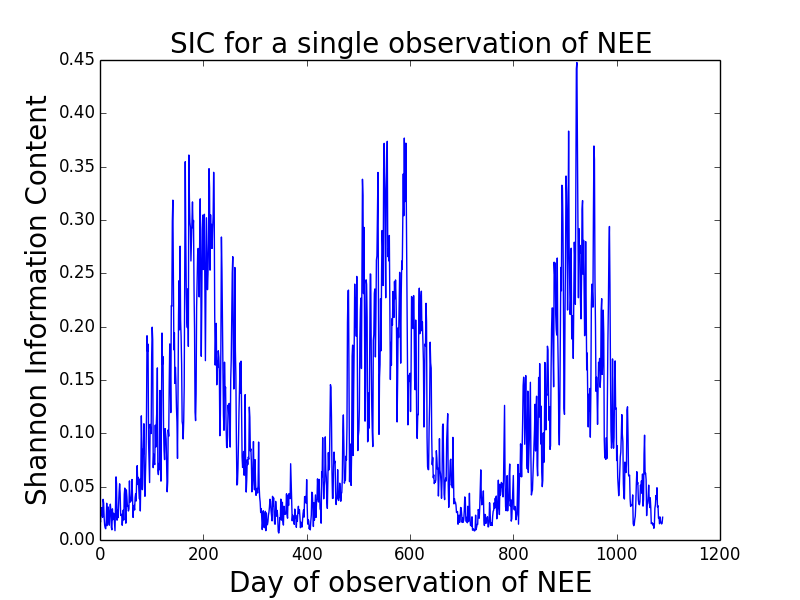
\includegraphics[width=.9\linewidth]{SIC1Obs_0_1095.png}
  \caption{$SIC$ for a single observation of $NEE$.}
  \label{fig:sub1}
\end{subfigure}%
\begin{subfigure}{.5\textwidth}
  \centering
  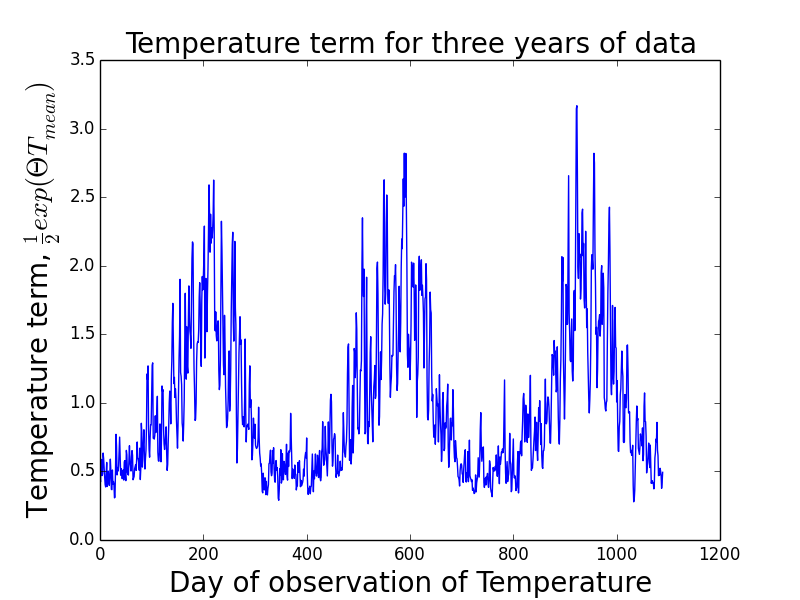
\includegraphics[width=.9\linewidth]{Temp_0_1095.png}
  \caption{Temperature term, $0.5exp(\Theta T_{mean})$.}
  \label{fig:sub2}
\end{subfigure}
\caption{$SIC$ and temperature varying over three years using driving data from Oregon pine forest.}
\label{fig:SICNEET}
\end{figure}

However the relationship is not linear as the magnitude of $GPP$'s first derivative is also dependent on daily irradiance and the value of the foliar carbon pool ($C_f$). This show that observations of $NEE$ made in the summer are much more valuable than those made in the winter assuming warmer temperatures, higher daily irradiance and a higher amount of foliar carbon in the summer.

\subsection*{$SIC$ for successive observations over a time window}

\begin{figure}[ht]
\centering
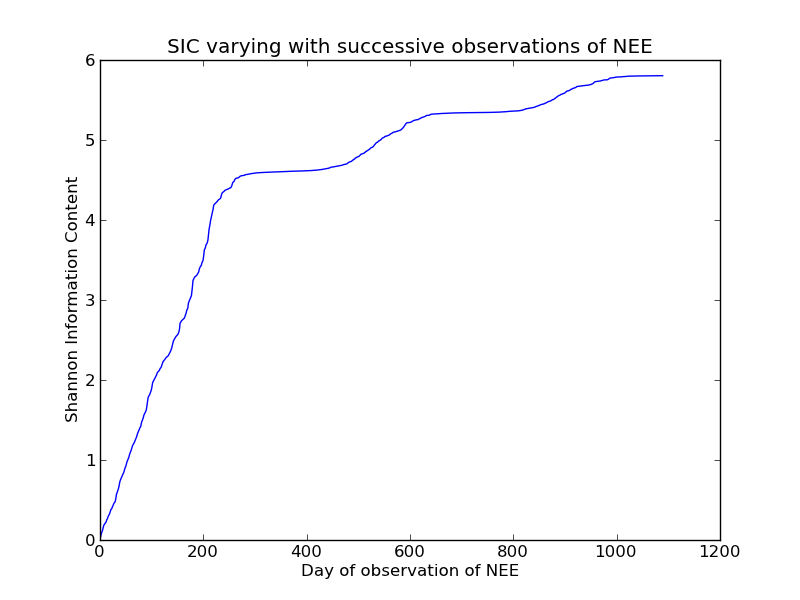
\includegraphics[width=1\textwidth]{SIC_0_1090.png}
\caption{$SIC$ varying as successive observations of $NEE$ are added using driving data from Oregon pine forest.}
\label{fig:SIC_subplot}
\end{figure} 

\begin{figure}[ht]
\centering
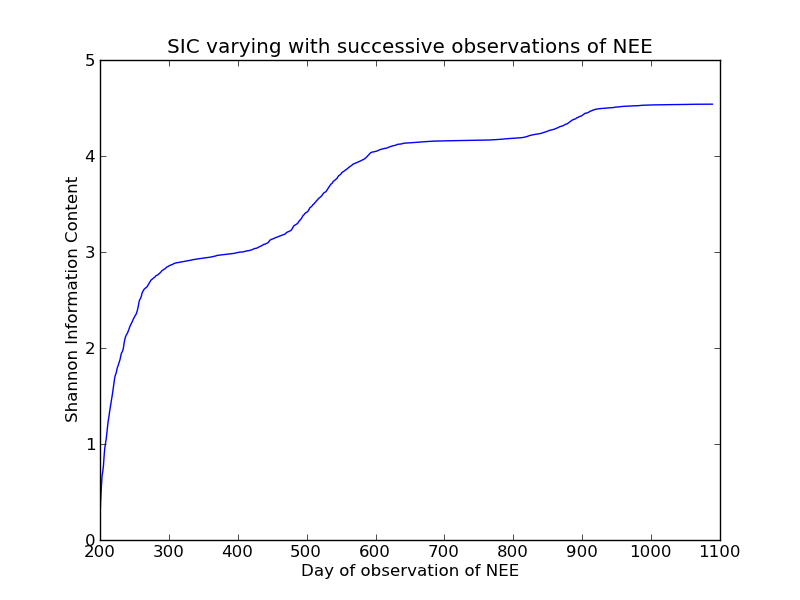
\includegraphics[width=1\textwidth]{SIC_200_1090.png}
\caption{$SIC$ varying as successive observations of $NEE$ are added using driving data from Oregon pine forest. Starting at day 200.}
\label{fig:SIC_subplot}
\end{figure}

\begin{figure}[ht]
\centering
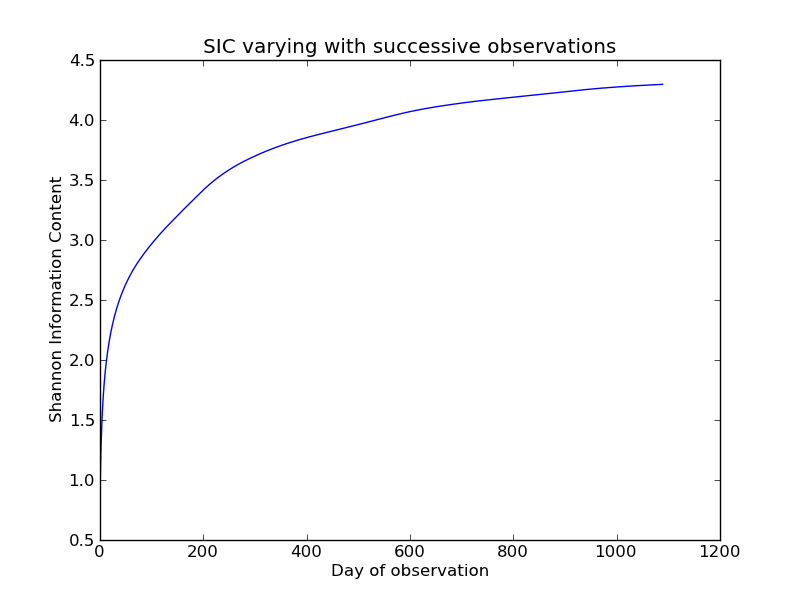
\includegraphics[width=1\textwidth]{SIC_0_1090Cf.png}
\caption{$SIC$ varying as successive observations of $Cf$ are added using driving data from Oregon pine forest.}
\label{fig:SIC_subplot}
\end{figure}

\begin{figure}[ht]
\centering
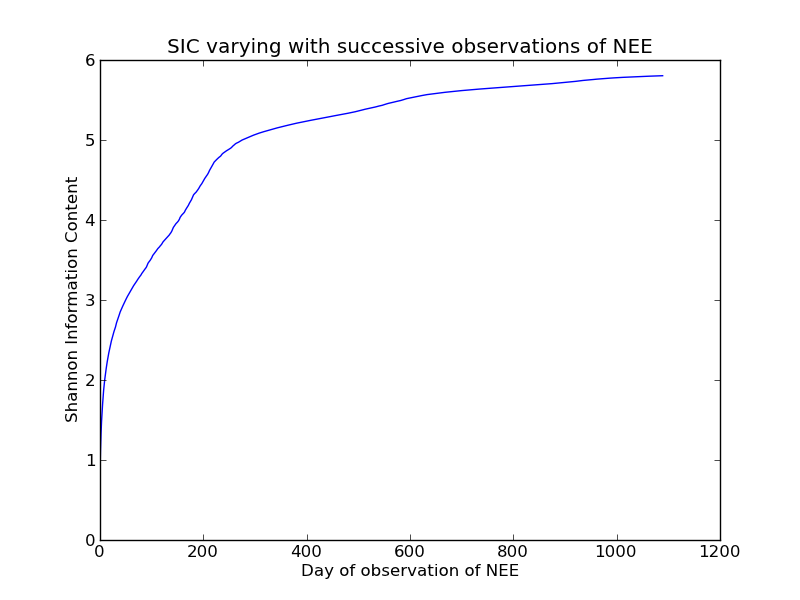
\includegraphics[width=1\textwidth]{SIC_0_1090CfNEE.png}
\caption{$SIC$ varying as successive observations of $NEE$ and $Cf$ are added using driving data from Oregon pine forest.}
\label{fig:SIC_subplot}
\end{figure}

\section*{Degrees of freedom for signal}

\[
DOFS==n-trace(\textbf{B}^{-1}\textbf{A})
\]

\begin{figure}[ht]
\centering
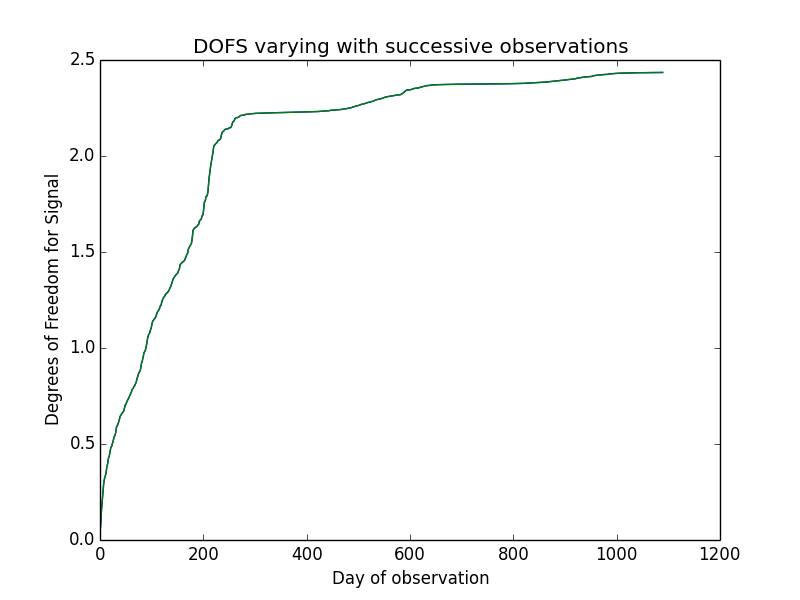
\includegraphics[width=1\textwidth]{DOFS_0_1090Cf_Cpoolsconst.png}
\caption{$DOFS$ varying as successive observations of $NEE$ are added using driving data from Oregon pine forest.}
\label{fig:SIC_subplot}
\end{figure}

\bibliography{../PhD}{}
\bibliographystyle{plain}
\end{document}
